\documentclass[a4paper,english,12pt]{article}
\usepackage{%
	amsfonts,%
	amsmath,%	
	amssymb,%
	amsthm,%
	algorithm,%
	babel,%
	bbm,%
	etex,%
	%biblatex,%
	caption,%
	centernot,%
	color,%
	dsfont,%
	enumerate,%
	epsfig,%
	epstopdf,%
	geometry,%
	graphicx,%
	hyperref,%
	latexsym,%
	mathtools,%
	multicol,%
	pgf,%
	pgfplots,%
	pgfplotstable,%
	pgfpages,%
	proof,%
	psfrag,%
	subfigure,%	
	tikz,%
	ulem,%
	url%
}	
\usepackage[noend]{algpseudocode}
\usepackage[mathscr]{eucal}
\usepgflibrary{shapes}
\usetikzlibrary{%
  	arrows,%
	backgrounds,%
	chains,%
	decorations.pathmorphing,% /pgf/decoration/random steps | erste Graphik
	decorations.text,%
	matrix,%
  	positioning,% wg. " of "
  	fit,%
	patterns,%
  	petri,%
	plotmarks,%
  	scopes,%
	shadows,%
  	shapes.misc,% wg. rounded rectangle
  	shapes.arrows,%
	shapes.callouts,%
  	shapes%
}

\theoremstyle{plain}
\newtheorem{thm}{Theorem}[section]
\newtheorem{lem}[thm]{Lemma}
\newtheorem{prop}[thm]{Proposition}
\newtheorem{cor}[thm]{Corollary}

\theoremstyle{definition}
\newtheorem{defn}[thm]{Definition}
\newtheorem{conj}[thm]{Conjecture}
\newtheorem{exmp}[thm]{Example}
\newtheorem{assum}[thm]{Assumptions}
\newtheorem{axiom}[thm]{Axiom}

\theoremstyle{remark}
\newtheorem{rem}{Remark}
\newtheorem{note}{Note}
\newtheorem{fact}{Fact}

\newcommand{\norm}[1]{\left\lVert#1\right\rVert}
\newcommand{\indep}{\!\perp\!\!\!\perp}
\DeclarePairedDelimiter\abs{\lvert}{\rvert}%
\newcommand\numberthis{\addtocounter{equation}{1}\tag{\theequation}}
\newcommand{\tr}{\operatorname{tr}}
\newcommand{\R}{\mathbb{R}}
\newcommand{\N}{\mathbb{N}}
\newcommand{\E}{\mathbb{E}}
\newcommand{\Z}{\mathbb{Z}}
\newcommand{\B}{\mathscr{B}}
\newcommand{\C}{\mathcal{C}}
\newcommand{\T}{\mathscr{T}}
\newcommand{\F}{\mathcal{F}}
\newcommand{\G}{\mathcal{G}}
%\newcommand{\ba}{\begin{align*}}
%\newcommand{\ea}{\end{align*}}
\DeclareMathOperator*{\argmax}{arg\,max}
\renewcommand{\qedsymbol}{$\blacksquare$}
\makeatletter
\def\BState{\State\hskip-\ALG@thistlm}
\makeatother

\makeatletter
\def\th@plain{%
  \thm@notefont{}% same as heading font
  \itshape % body font
}
\def\th@definition{%
  \thm@notefont{}% same as heading font
  \normalfont % body font
}
\makeatother
\date{}

\begin{document}
\title{Lecture 24: LINEAR MMSE ESTIMATION THEORY}
\author{}
\date{05 April 2016}
\maketitle
In the previous lecture, we dealt with \textit{Kalman-Bucy} filter which is the recursive/sequential algorithm to output the optimal MMSE state of a linear dynamical system with Gaussian statistics. Recursive relations for the above algorithm were derived. In this lecture, we will discuss the general theory of linear estimation which reduces computational complexity. Orthogonality principle, it's alternative version will be proved and \textit{Levinson-Durbin} filter will be introduced. 
\section{Linear MMSE Estimation Theory}
Suppose we have two real valued discrete time random processes 
$\{X_n\}_{n=0}^\infty$ \& $\{Y_n\}_{n=0}^\infty$ and we want to estimate $X_t$ using the observations $(Y_0,Y_1,....,Y_s)$ to minimize mean square error(MSE) i.e., $\mathbb{E}[(X_t-\hat{X_t})^2]$. The optimum estimator in the MMSE sense is  the conditional mean of $X_t$
\begin{equation}
\hat{X_t}=\mathbb{E}[X_t|Y_1,Y_2,...,Y_s].
\end{equation}
However, if the number of observations are large then computation of conditional mean is quite cumbersome, unless the problem exhibits special structure (as in \textit{Kalman-Bucy} model).
\par Computational complexity of these problems can be reduced by constrained estimators. One such class of constraints is linear constraint, where the estimate is linear function of $(Y_0,Y_1,...,Y_s)$, i.e., functions of the form 
\begin{equation}
\hat{X_t}=\sum_{n=1}^s h_nY_n+h_0.
\end{equation}
Let $\mathcal{H}^s$ denote the set of all linear estimators, such that
\begin{equation}
\{\hat{X_t}:\hat{X_t}=\sum_{n=1}^s h_nY_n+h_0\}\label{eq1}.
\end{equation}
Consider the best linear estimator problem 
\begin{equation}
\mbox{minimize}~\mathbb{E}[(X_t-\hat{X_t})^2]~~\mbox{s.t}~~\hat{X_t}\in \mathcal{H}^s. \label{eq2}
\end{equation}
\begin{thm}{(Orthogonality Principle)}\\
Consider the best linear estimation problem as in eqn. \eqref{eq2}. $\hat{X_t}\in \mathcal{H}^s$ solves the problem if and only if $\mathbb{E}[(\hat{X_t}-X_t)Z]=0,~~\forall~~Z \in \mathcal{H}^s$.
\end{thm}
\begin{proof}
Assume that $\mathbb{E}[(\hat{X_t}-X_t)Z]=0 \; \forall Z \in \mathcal{H}^s$.
Let $\tilde{X_t}\in \mathcal{H}^s$ be any linear estimator.
\begin{align}
\mathbb{E}[(\tilde{X_t}-X_t)^2]&=\mathbb{E}[(\tilde{X_t}-\hat{X_t}+\hat{X_t}-X_t)^2],
\nonumber\\
&=\mathbb{E}[(\tilde{X_t}-\hat{X_t})^2]+\mathbb{E}[(\hat{X_t}-X_t)^2]+2\mathbb{E}[(\tilde{X_t}-\hat{X_t})(\hat{X_t}-X_t)],
\nonumber\\
&=\underbrace{\mathbb{E}[(\tilde{X_t}-\hat{X_t})^2]}_{\geqslant0}+\underbrace{\mathbb{E}[(\hat{X_t}-X_t)^2]}_{\geqslant0}+ \underbrace{2\mathbb{E}[(\tilde{X_t}-\hat{X_t})(\hat{X_t}-X_t)]}_{=0} \label{eq3},\\
&\geq \mathbb{E}[(\hat{X_t}-X_t)^2].
\nonumber
\end{align}
The third term in the equation \eqref{eq3} is zero since $\mathbb{E}[(\hat{X_t}-X_t)Z]=0$, where $Z=\tilde{X_t}-\hat{X_t}$ (difference of two linear estimators) is also a linear estimator. Assume that $\tilde{X_t}\in \mathcal{H}^s$, $Z \in \mathcal{H}^s$ such that $\mathbb{E}[(\tilde{X_t}-X_t)Z]\neq0$.
We will construct a better estimator than $\tilde{X_t}$. Define
\begin{align}
\nonumber
\hat{X_t}&=\tilde{X_t}-\left[\frac{\mathbb{E}[(\tilde{X_t}-X_t)Z]Z}{\mathbb{E}[Z^2]}\right]=\tilde{X_t}-\left[\frac{aZ}{b}\right] ,
\end{align}
where $a=\mathbb{E}[(\tilde{X_t}-X_t)Z] \; \text {and} \; b=\mathbb{E}[Z^2]$.
\begin{align}
\mathbb{E}[(\tilde{X_t}-X_t)^2]&=\mathbb{E}[(\tilde{X_t}-\frac{aZ}{b}-X_t)^2],\nonumber\\
&=\mathbb{E}[(\tilde{X_t}-X_t)^2]+\frac{a^2}{b^2}\mathbb{E}[Z^2]-2\frac{a}{b}\mathbb{E}[(\tilde{X_t}-X_t)Z)],\nonumber\\
&=\mathbb{E}[(\tilde{X_t}-X_t)^2]+\frac{a^2}{b}-\frac{2a^2}{b},\nonumber\\
&=\mathbb{E}[(\tilde{X_t}-X_t)^2]-\frac{a^2}{b}\nonumber,\\
&\leq \mathbb{E}[(\tilde{X_t}-X_t)^2].
\nonumber
\end{align}
Hence orthogonality principle is proved.
\end{proof}
\begin{figure}
\centering
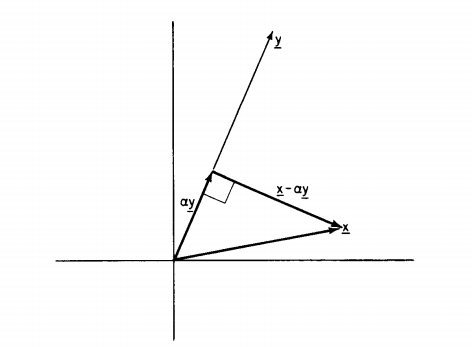
\includegraphics[scale=1]{Figures/Lec24_fig1.png}
\caption{Illustration of Orthogonality Principle for 1-dimension}\label{fig:fig1}
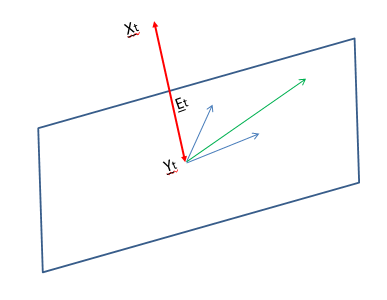
\includegraphics[scale=1]{Figures/Lec24_fig2.png}
\caption{Illustration of Orthogonality Principle for 2-dimensions}\label{fig:fig2}
\end{figure}
\pagebreak
Suppose that $\underline{x}$ and $\underline{y}$ are two vectors of same dimension, and suppose that we would like to approximate $\underline{x}$ by a constant, say $\alpha$, times $\underline{y}$ such that length of error vector $\underline{x}-\alpha\underline{y}$ is as small as possible. It is is easy to see that $\alpha$ minimizes this length if and only if error vector is perpendicular to the line that is along $\underline{y}$ (see Fig. \ref{fig:fig1}).
In Fig. \ref{fig:fig2}, the plane shows the subspace of $\mathcal{H}^s$, $\underline{Y}_t$ is the LMMSE estimate of $\underline{X}_t$, since error vector $\underline{E}_t=(\underline{Y}_t-\underline{X}_t)$ is perpendicular to the plane. 
%\pagebreak
\begin{thm}\label{thm:thm2}
Another Orthogonality Principle:
$ \hat{X}_t \in \mathcal{H}^s $ solves eqn. \eqref{eq2} iff $
 \mathbb{E}[\hat{X}_{t}]=\mathbb{E}[X_{t}]$  and 
 $\mathbb{E}[(\hat{X}_{t}-X_t)Y_l]=0$, $\forall \; l=1,2,3,...,s$.
\end{thm}
\begin{flushleft}
This is an alternative orthogonality condition.
\end{flushleft}
\subsection{Explicit Solution for the Optimal LMMSE \\ Estimator}
Assume that the best linear estimator of $X_t$ given $(Y_1,....,Y_s)$ is
\begin{align}
	\hat{X}_t=\sum_{n=1}^s h_nY_n+h_0.
\end{align}
From theorem \ref{thm:thm2}, we have
\begin{align}
\mathbb{E}[\hat{X}_{t}]=\sum_{n=1}^{s}{h_n\mathbb{E}[Y_n]}+h_0=\mathbb{E}[X_{t}].
\end{align}
This gives,
\begin{align}
h_0=\mathbb{E}[X_t]-
 \sum_{n=1}^{s}{h_n\mathbb{E}[Y_{n}]}.\label{eq4}  
\end{align}
Also, for all $l=1,\dots,s$,
\begin{equation}
  \mathbb{E}\left\lbrace\left(X_{t}-\underbrace{\left[\sum_{n=1}^{s}{h_nY_n}+h_0\right]}_{\hat{X}_t}\right)Y_l\right\rbrace = 0\label{eq5}
\end{equation}  
Substituting eqn. \eqref{eq4} in eqn. \eqref{eq5}, we get
 \begin{align}
\mathbb{E}\left\lbrace\left((X_{t}-\mathbb{E}[X_t])-\sum_{n=1}^{s}h_n(Y_n-\mathbb{E}\lbrace Y_n \rbrace)\right)Y_l\right\rbrace&=0, 
\end{align}
\begin{align}
\mathbb{E}[(X_{t}-X_t)Y_l]&=
\sum_{n=1}^{s}h_n\mathbb{E}\left[\left(Y_n-\mathbb{E}\lbrace Y_n \rbrace\right)Y_l\right], \nonumber \\
\text{Cov}(X_t,Y_l)&=\sum_{n=1}^{s} h_n\text{Cov}(Y_n,Y_l), \; \forall\; 1\leq l \leq s, \nonumber\\
C_{XY}(t,l)&=\sum_{n=1}^{s} h_nC_Y(n,l), \; \forall \; 1\leq l
\leq s.
\end{align}
%\begin{flushleft}
the above equations are called \textit{Yule-Walker Equations (or) Weiner-Hopf Equations},
%\end{flushleft}
where
$C_{XY}(t,l) \overset{\Delta}{=} \text{Cov}(X_t,Y_l)$ is the cross covariance function of 
$\{ X_n \}_{n=0}^{\infty}$ and $\{ Y_n \}_{n=0}^{\infty} $ and  $C_Y(n,l)\overset{\Delta}{=} \text{Cov}(Y_n,Y_l)$ is the auto covariance function of the sequence  $\{ Y_n \}_{n=0}^{\infty} $.
\begin{note}
First and second order statistics of $X$ and $Y$ completely determine the optimal Linear Estimator.
\end{note}
In Matrix form,
\begin{equation}
\underline{\sigma}_{XY} = \Sigma_Y \underline{h} \nonumber,
\end{equation} 
where
\begin{eqnarray}
\underline{\sigma}_{XY} & \overset{\Delta}{=} & [C_{XY}(t,l),.....,C_{XY}(t,s)]^T,\nonumber \\
\underline{h} & \overset{\Delta}{=} & [h_{t,1},.......,h_{t,s}]^T. \nonumber
\end{eqnarray}
If $\Sigma_{Y}$ is positive definite, then the optimum estimator coefficients are given by
\begin{center}
$\underline{h} =  \Sigma_{Y}^{-1}\underline{\sigma}_{XY}.$
\end{center}
\begin{note}
Inverting $\Sigma_Y$ of size $s \times s$ is expensive, if $s$ is large (in general, time required for inversion of $\Sigma_{Y}$ is $O(s^3)$. In our case $s$ is the number of observations, which grows linearly with time for many signal estimation applications. So, the computation of optimum coefficients from above equation cannot be accomplished in real time.
\end{note}
\par However, with more structure in the problem, one can hope to solve it faster.
The following models provide more efficient computation of these coefficients.
\begin{enumerate}
\item Kalman filter for linear dynamical systems.
\item Levinson-Durbin filter for wide sense stationary processes (WSSP).
\end{enumerate}
\section{Levinson-Durbin Filter}
Suppose $\{Y_n\}_{n=0}^\infty$ is a wide sense stationary random process with zero mean and auto-covariance function $C_Y(n,l)=C_Y(n-l,0)=C_Y(n-l)$. At each time $t=1,2,...$, we want to output best linear estimate of $Y_{t+1}$ using $(Y_0,Y_1,Y_2,....,Y_t)$. In the previous notation $X_t \leftrightarrow Y_{t+1}$ and $s \leftrightarrow t$.
\begin{align}
C_{XY}&=\text{Cov}(X_t,Y_l), \nonumber\\
&=\text{Cov}(Y_{t+1},Y_l), \nonumber\\
&=C_Y(t+1-l). \nonumber
\end{align}
\subsection{Yule-Walker Equations}
Let the optimal estimator be $\hat{Y}_{t+1}=\sum_0^t h_{t,n}Y_n.$
\begin{equation}
\begin{bmatrix}
C_Y(t+1)\\
C_Y(t)\\
. \\
. \\
C_Y (1)
\end{bmatrix}
=
\underbrace{\begin{bmatrix}
C_Y(0) & C_Y(1) & .& .& .& C_Y(t)\\
C_Y(1) & C_Y(2) & .&. & .& C_Y(t-1)\\ 
. & .& & &  & .&  \\
. & .& & &  & .&  \\
C_Y(t) & C_Y(t-1) & .& .& .& C_Y(0) 
\end{bmatrix}}_{\Sigma_Y}
\begin{bmatrix}
h_{t,0} \\
h_{t,1}\\
.\\
.\\
h_{t,t} 
\end{bmatrix} \label{eq6}
\end{equation}
The matrix $\Sigma_Y$ in the eqn. \eqref{eq6} is a \textit{Toeplitz}
matrix, which means that its entries are constant along the diagonals (since $C_Y(n,l)=C_Y(n-l)$).
\end{document}